\laatikko{Eräs tärkeä yhtälöiden tyyppi ovat \termi{potenssiyhtälö}{potenssiyhtälöt}.

Potenssiyhtälö on muotoa $x^n=a$,
oleva yhtälö, jossa $n$ on positiivinen kokonaisluku.
Eksponentin $n$ arvoa kutsutaan potenssiyhtälön \termi{aste (potenssiyhtälö)}{asteeksi}.

Potenssiyhtälöitä tarvitaan esimerkiksi tilanteissa, joissa lasketaan korolle korkoa.
Myös pinta-ala- ja tilavuuslaskuissa esiintyy potenssiyhtälöitä.}

\begin{esimerkki}
	\begin{alakohdat}
		\alakohta{Yhtälö $27x^3=7$ on potenssiyhtälö, sillä jakamalla se puolittain luvulla $27$ saadaan $x^3 = \frac{7}{27}$.}
		\alakohta{Yhtälö $2x^{4}-7=3$ on potenssiyhtälö, sillä se voidaan muokata muotoon $x^n = a$,
			\begin{eqnarray*}
				2x^{4} -7 &=& 3 \\
				2x^{4} &=& 3+7 \\
				x^{4} &=& \frac{10}{2} \\
				x^{4} &=& 5.
			\end{eqnarray*}}
		\alakohta{Yhtälö $x^{\frac{3}{2}}=42$ ei ole potenssiyhtälö, sillä eksponentti $\frac{3}{2}$ ei ole kokonaisluku. Yhtälö voidaan kuitenkin kirjoittaa uuden tuntemattoman $z=x^{\frac{1}{2}}=\sqrt{x}$ avulla: tällöin saadaan potenssiyhtälö $z^3 = 42$.)}
		\alakohta{Yhtälö $x^{-2}=44$ ei ole potenssiyhtälö, sillä $-2$ ei ole positiivinen kokonaisluku. Sekin voidaan kirjoittaa potenssiyhtälönä, kun merkitään $z=x^{-1}=\frac{1}{x}$. Tällöin saadaan yhtälö $z^2 = 44$.)}
	\end{alakohdat}
\end{esimerkki}

\laatikko{Potenssiyhtälön ratkaiseminen:
	\begin{alakohdat}
		\alakohta{Jos potenssiyhtälön aste $n$ on parillinen ja $a \ge 0$, yhtälöllä on kaksi ratkaisua, $$ x = \pm \sqrt[n]{a} \textrm{.} $$ ($\pm$ tarkoittaa, että sekä positiivinen että negatiivinen arvo käyvät: $\pm 5$ tarkoittaa sekä lukuja $5$ että $-5$.)}
		\alakohta{Jos aste on pariton, yhtälöllä on täsmälleen yksi ratkaisu,$ x = \sqrt[n]{a}.$}
		\alakohta{Jos aste on parillinen ja $a < 0$, potenssiyhtälöllä ei ole yhtään ratkaisua.}
	\end{alakohdat}
}

\begin{esimerkki}
	\begin{alakohdat}
		\alakohta{Potenssiyhtälön $x^3 = 100$ ratkaisu on $x=\sqrt[3]{100}$.}
		\alakohta{Potenssiyhtälöllä $x^4=50$ on kaksi ratkaisua $x=\sqrt[4]{50}=2{,}6591...$ ja $x=-\sqrt[4]{50}=-2{,}6591...$.}
		\alakohta{Potenssiyhtälöllä $x^6 = -1$ ei ole ratkaisua, sillä $x^6 = (x^3)^2 \ge 0$ kaikilla $x$.}
	\end{alakohdat}
	\begin{center}
		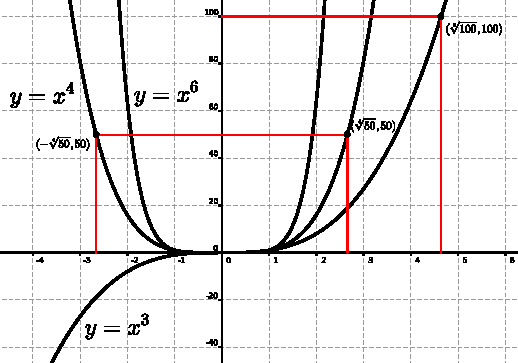
\includegraphics[width=11.5cm]{pictures/xpot346.pdf} %KUVAAJILLE ERI VÄRIT SELVENTÄISI ASIAA
	\end{center}
\end{esimerkki}


\begin{esimerkki}
	Suursijoittaja Nalle Mursulla on $5~000$ euroa ylimääräistä rahaa, jonka hän aikoo sijoittaa $30$ vuodeksi.  Nalle Mursu haluaa sijoittamansa pääoman kasvavan $100~000$ euroksi $30$ vuodessa.  Kuinka suuren vuotuisen korkokannan Nalle Mursu tarvitsee sijoitukselleen? 
	\begin{esimratk}
		Olkoon vuotuinen korkokanta $r$. Korkoa korolle -periaatteen nojalla $5~000$ euron sijoitus
		kasvaa $30$ vuodessa summaksi $5~000\cdot(1+r)^{30}$. Merkitsemällä $x=1+r$ saamme yhtälön $5~000\cdot x^{30} = 100~000$.
		Jakamalla yhtälö puolittain luvulla $5~000$ päädymme potenssiyhtälöön
		\[ x^{30} = 20, \] 
		jonka ratkaisuksi saadaan $x=20^{\frac{1}{30}} = 1{,}105\ldots$. Näin
		ollen suursijoittaja Nalle Mursun vaatima korkokanta sijoitukselleen on noin $r=1-x=1-1,105=0,105=10{,}5~\%$.
	\end{esimratk}
\end{esimerkki}

\laatikko{Mikäli potenssiyhtälön asteluku $n$ on pariton, yhtälöllä on aina tasan yksi ratkaisu (kun $a \neq 0$).}

\begin{esimerkki}
Ratkaise yhtälö $2x^3 + 16 = 0$

	$2x^3 + 16 = 0 \\
	2x^3 = -16 \\
	x^3 = -8  \\
	x = \sqrt[3]{-8} = -2 $
\end{esimerkki}

\laatikko{Mikäli potenssiyhtälön asteluku $n$ on parillinen, yhtälö on ratkaistavissa jos ja vain jos $\frac{b}{a} \geq 0 $. Parillisella potenssifunktiolla voi olla yksi, kaksi tai ei yhtään ratkaisua.}

\begin{esimerkki}
Ratkaise yhtälöt a) $x^2 = 0$, b) $x^2 - 9 = 0$ ja c) $x^2 + 9 = 0$

a)	$x^2 = 0 \\
	x = 0 \\$
	Yhtälöllä on yksi ratkaisu $x = 0$.

b)	$x^2 - 9 = 0 \\
	x^2 = 9 \\
	x = \pm 3 \\$
	Yhtälöllä on kaksi ratkaisua $x = 3$ ja $x = -3$, sillä $3^2 = 9$ ja $(-3)^2 = 9$.

c)	$x^2 + 9 = 0 \\
	x^2 = -9 \\
	x = \sqrt{-9} \\$
	Yhtälöllä ei ole reaalista ratkaisua.

\end{esimerkki}